\documentclass[aspectratio=43,11pt]{beamer}

% =========================================================
% Encoding and Fonts
% =========================================================
\usepackage[utf8]{inputenc}
\usepackage[T1]{fontenc}

% =========================================================
% Packages
% =========================================================
\usepackage{booktabs}
\usepackage{array}
\usepackage{graphicx}
\usepackage{soul}
\usepackage{tikz}

\usetikzlibrary{
    arrows.meta,
    positioning
}

% =========================================================
% Beamer Theme and Layout
% =========================================================
\usetheme{default}
\usecolortheme{default}

% Remove navigation icons
\setbeamertemplate{navigation symbols}{}

% Show frame number in footer
\setbeamertemplate{footline}[frame number]

% =========================================================
% Custom Colors
% =========================================================

% Texas A&M Aggie Maroon
\definecolor{aggiemaroon}{RGB}{80,0,0}

% Main presentation colors
\setbeamercolor{title}{fg=aggiemaroon}
\setbeamercolor{frametitle}{fg=aggiemaroon}
\setbeamercolor{section in toc}{fg=aggiemaroon}
\setbeamercolor{subsection in toc}{fg=aggiemaroon}
\setbeamercolor{subsubsection in toc}{fg=aggiemaroon}
\setbeamercolor{section number projected}{bg=aggiemaroon,fg=white}
\setbeamercolor{subsection number projected}{bg=aggiemaroon,fg=white}

% =========================================================
% Typography
% =========================================================

% Font sizes tuned for 4:3 slides
\setbeamerfont{title}{size=\Large}
\setbeamerfont{subtitle}{size=\normalsize}
\setbeamerfont{frametitle}{size=\large}

% =========================================================
% Itemize Lists
% =========================================================

% Bullet colors
\setbeamercolor{itemize item}{fg=aggiemaroon}
\setbeamercolor{itemize subitem}{fg=aggiemaroon}
\setbeamercolor{itemize subsubitem}{fg=aggiemaroon}

\setbeamertemplate{itemize items}[circle]

% Bullet symbols
%\setbeamertemplate{itemize item}{\textbullet}
%\setbeamertemplate{itemize subitem}{\textbullet}
%\setbeamertemplate{itemize subsubitem}{\textbullet}

% =========================================================
% Enumerated Lists
% =========================================================

\setbeamercolor{enumerate item}{fg=aggiemaroon}
\setbeamercolor{enumerate subitem}{fg=aggiemaroon}

\setbeamertemplate{enumerate item}{(\insertenumlabel)}
\setbeamertemplate{enumerate subitem}{(\insertsubenumlabel)}

% =========================================================
% Presentation Information
% =========================================================

\title{
    Data Requirements, Data Provenance,\\
    and Acquisition Strategies
}

\author{}

\date{
    \textcolor{aggiemaroon}{
        DAEN 459 -- Fall 2026\\
        \textbf{Alexander Abuabara}
    }
}

% =========================================================
% Title Page Graphic
% =========================================================

\titlegraphic{
    \vfill
    
\includegraphics[height=1.2cm]{TAMU_logo.png}
}

\begin{document}

%---------------------------------------------------------------
\begin{frame}
  \titlepage
\end{frame}

%---------------------------------------------------------------
\begin{frame}{Outline}
  \tableofcontents
\end{frame}

%---------------------------------------------------------------
\section{Example}

\begin{frame}{Example: Bike-Share Pipeline}
  \textbf{Capstone goal:} build a pipeline that delivers clean, documented,
  analysis-ready data for forecasting hourly bike demand per station.

  \medskip
  \textbf{Candidate sources}
  \begin{itemize}
    \item Trip records (monthly CSV dumps from the operator)
    \item Live station status (GBFS JSON API)
    \item Weather (public API, hourly)
    \item City events calendar (web page, semi-structured)
    \item Census tract demographics (annual release)
  \end{itemize}

  \medskip
  \textbf{Downstream consumers:} a forecasting model, a dashboard, and a
  monthly report to the city.
\end{frame}

%---------------------------------------------------------------
\section{Data Requirements}

\begin{frame}{Why Requirements Come First}
  \begin{itemize}
    \item Requirements are derived from \alert{decisions and questions}, not
      from whatever data happens to be available.
    \item Poorly specified requirements lead to rework, scope creep, and
      models trained on the wrong grain of data.
    \item Capture requirements as testable statements that can be checked
      automatically later.
  \end{itemize}

  \medskip
  \textbf{Chain of reasoning}

  \medskip
  \resizebox{\textwidth}{!}{%
  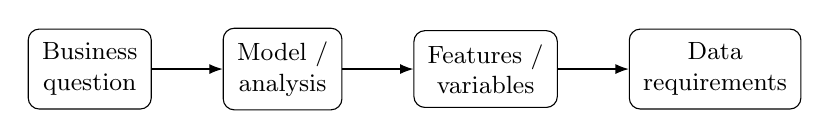
\begin{tikzpicture}[node distance=0.9cm, every node/.style={draw, rounded corners, align=center, font=\small, inner sep=5pt}]
    \node (q) {Business\\question};
    \node (m) [right=of q] {Model /\\analysis};
    \node (f) [right=of m] {Features /\\variables};
    \node (d) [right=of f] {Data\\requirements};
    \draw[-{Latex}] (q) -- (m);
    \draw[-{Latex}] (m) -- (f);
    \draw[-{Latex}] (f) -- (d);
  \end{tikzpicture}}
\end{frame}

\begin{frame}{Dimensions of a Data Requirement}
  \small
  \begin{tabular}{@{}p{3.0cm}p{7.1cm}@{}}
    \toprule
    \textbf{Dimension} & \textbf{Question to answer} \\
    \midrule
    Content & Which entities and attributes are needed? \\
    Granularity & Per trip, per station-hour, per day? \\
    Coverage & Which time span, stations, geography? \\
    Volume \& velocity & Rows per day? Batch or streaming? \\
    Quality & Acceptable missingness, error rate, duplicates? \\
    Timeliness & How stale can the data be? \\
    Access \& legal & Licenses, privacy, retention limits? \\
    \bottomrule
  \end{tabular}
\end{frame}

\begin{frame}{Example: Testable Requirements}
  \footnotesize
  \begin{tabular}{@{}p{5.1cm}p{5.1cm}@{}}
    \toprule
    \textbf{Requirement} & \textbf{Acceptance check} \\
    \midrule
    R1: Station-hour demand for 36 months & No gaps longer than 2 hours per station \\[3pt]
    R2: Weather joined at station-hour & $\geq 98\%$ of rows have temperature and precipitation \\[3pt]
    R3: Station IDs consistent across sources & 100\% of trip station IDs exist in the station dimension \\[3pt]
    R4: Forecast inputs refreshed daily by 06:00 & Pipeline SLA monitor; alert if late \\[3pt]
    R5: No rider-level PII stored & Schema scan finds no user ID or birth year \\
    \bottomrule
  \end{tabular}

  \normalsize
  \medskip
  Each requirement maps to an automated data-quality test in the pipeline.
\end{frame}

\begin{frame}{Example: Gaps Found Early}
  \begin{itemize}
    \item The forecasting model needs \textbf{station-hour} counts.
    \item Trip files record \textbf{trip start/end timestamps}, so counts must be
      derived by aggregation.
    \item \alert{Gap found:} rebalancing trips (staff moving bikes) are not labeled,
      so they inflate demand.
    \item \textbf{Action:} add a requirement to identify or filter rebalancing
      events, and ask the operator whether a flag exists.
  \end{itemize}
\end{frame}

%---------------------------------------------------------------
\section{Data Provenance}

\begin{frame}{What Is Data Provenance?}
  \textbf{Provenance} is the \hl{recorded history of a dataset}: where it came from,
  who or what transformed it, and when.

  \medskip
  \begin{itemize}
    \item \textbf{Origin:} source system, URL, owner, license
    \item \textbf{Process:} code version, parameters, environment
    \item \textbf{Lineage:} the chain of datasets and transformations to the
      final output
    \item \textbf{Time:} extraction time and the period the data describes
  \end{itemize}

  \medskip
  Why it matters: reproducibility, debugging, auditing, trust, and
  compliance.
\end{frame}

\begin{frame}{Lineage Diagram for the Example}
  \resizebox{\textwidth}{!}{%
  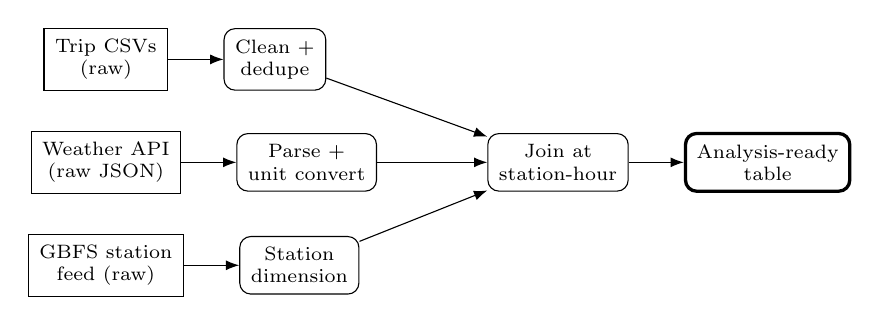
\begin{tikzpicture}[
      node distance=0.5cm and 0.7cm,
      src/.style={draw, rectangle, align=center, font=\scriptsize, inner sep=4pt},
      proc/.style={draw, rounded corners, align=center, font=\scriptsize, inner sep=4pt},
      outbox/.style={draw, very thick, rounded corners, align=center, font=\scriptsize, inner sep=4pt}]
    \node[src] (trips) {Trip CSVs\\(raw)};
    \node[src, below=of trips] (wx) {Weather API\\(raw JSON)};
    \node[src, below=of wx] (gbfs) {GBFS station\\feed (raw)};
    \node[proc, right=of trips] (ctrips) {Clean +\\dedupe};
    \node[proc, right=of wx] (cwx) {Parse +\\unit convert};
    \node[proc, right=of gbfs] (cst) {Station\\dimension};
    \node[proc, right=1.4cm of cwx] (join) {Join at\\station-hour};
    \node[outbox, right=of join] (mart) {Analysis-ready\\table};
    \draw[-{Latex}] (trips) -- (ctrips);
    \draw[-{Latex}] (wx) -- (cwx);
    \draw[-{Latex}] (gbfs) -- (cst);
    \draw[-{Latex}] (ctrips) -- (join);
    \draw[-{Latex}] (cwx) -- (join);
    \draw[-{Latex}] (cst) -- (join);
    \draw[-{Latex}] (join) -- (mart);
  \end{tikzpicture}}

  \medskip
  Every arrow should be traceable to a versioned script and a logged run.
\end{frame}

\begin{frame}[fragile]{Provenance Metadata Record}
  Store a small metadata file next to every raw extract:

  \medskip
  \footnotesize
\begin{verbatim}
source_name:    weather_hourly_api
source_url:     https://api.example.org/v1/hourly
license:        CC-BY-4.0
retrieved_at:   2026-10-04T05:12:09-05:00
period_covered: 2026-10-03T00:00 / 2026-10-03T23:00
request_params: {lat: 30.62, lon: -96.33, units: metric}
raw_file:       raw/weather/2026-10-03.json
sha256:         9f2c...e41a
code_version:   git commit 3b7d1a2
\end{verbatim}

  \normalsize
  A checksum plus a commit hash lets anyone verify that a result came from a
  specific input and a specific version of the code.
\end{frame}

\begin{frame}{Provenance Practices for a Capstone}
  \begin{itemize}
    \item Keep raw data \textbf{immutable}; never edit in place.
    \item Separate layers: \texttt{raw} $\rightarrow$ \texttt{clean} $\rightarrow$
      \texttt{curated}.
    \item Version code in Git; record the commit in each run's metadata.
    \item Pin environments (\texttt{requirements.txt}, \texttt{renv.lock}, or a
      container image).
    \item Keep a data dictionary and a changelog of schema changes.
    \item Use workflow tools (e.g., Make, Snakemake, Airflow, dbt) so lineage is
      declared, not remembered.
  \end{itemize}
\end{frame}

\begin{frame}{Example: Provenance Saves the Day}
  \textbf{Symptom:} Forecast error jumps in March.

  \medskip
  \textbf{Investigation using provenance records}
  \begin{enumerate}
    \item Compare run metadata: the weather source changed its temperature
      unit from Celsius to Fahrenheit on March 1.
    \item Raw files confirm the change; the parsing step assumed Celsius.
    \item Fix the parser, add a unit-validation test, and reprocess from
      immutable raw files.
  \end{enumerate}

  \medskip
  Without raw snapshots and recorded parameters, the root cause would be
  hard to prove and the data impossible to rebuild.
\end{frame}

%---------------------------------------------------------------
\section{Acquisition Strategies}

\begin{frame}{Acquisition Options}
  \footnotesize
  \begin{tabular}{@{}p{2.4cm}p{3.3cm}p{4.0cm}@{}}
    \toprule
    \textbf{Strategy} & \textbf{Example} & \textbf{Main trade-off} \\
    \midrule
    Bulk download & Monthly trip CSVs & Simple, but latency and format drift \\[3pt]
    API pull & Hourly weather & Structured, but rate limits and auth \\[3pt]
    Streaming feed & GBFS station status & Fresh, but needs durable storage \\[3pt]
    Web scraping & City events page & Fragile; check terms of use \\[3pt]
    Purchase / partner & Operator data agreement & Rich, but cost and legal terms \\[3pt]
    Generate / simulate & Synthetic trips for testing & Safe, but may not match reality \\
    \bottomrule
  \end{tabular}
\end{frame}

\begin{frame}{Choosing a Strategy: Decision Factors}
  \begin{itemize}
    \item \textbf{Fit to requirements:} does it satisfy granularity, coverage, and timeliness?
    \item \textbf{Reliability:} uptime, versioning, documented schema, stable identifiers.
    \item \textbf{Cost and effort:} licensing fees, engineering time, storage.
    \item \textbf{Legal and ethical:} license, terms of service, privacy, consent.
    \item \textbf{Risk:} single point of failure, vendor lock-in, source discontinuation.
  \end{itemize}

  \medskip
  Score each candidate source against these factors before committing.
\end{frame}

\begin{frame}{Example: Source Evaluation Matrix}
  \footnotesize
  \begin{tabular}{@{}lllll@{}}
    \toprule
    \textbf{Source} & \textbf{Fit} & \textbf{Reliability} & \textbf{Cost} & \textbf{Legal} \\
    \midrule
    Trip CSVs & High & High & Free & Open \\
    Weather API A & High & High & Free tier & Attribution \\
    Weather API B & Medium & Medium & Paid & Restrictive \\
    Events scraping & Medium & Low & Free & Unclear \\
    Census tables & Medium & High & Free & Public domain \\
    \bottomrule
  \end{tabular}

  \normalsize
  \medskip
  \textbf{Decision:} use Trip CSVs, Weather API A, and Census; treat events
  scraping as optional and defer until the baseline pipeline works.
\end{frame}

\begin{frame}[fragile]{Example: Resilient API Acquisition}
  Retries with backoff, raw payload storage, and logged metadata:

  \medskip
  \scriptsize
\begin{verbatim}
import requests, time, json, hashlib, datetime as dt

def fetch(url, params, retries=4):
    for k in range(retries):
        r = requests.get(url, params=params, timeout=30)
        if r.status_code == 200:
            return r.content
        time.sleep(2 ** k)          # exponential backoff
    raise RuntimeError("fetch failed")

payload = fetch(URL, PARAMS)
path = f"raw/weather/{dt.date.today()}.json"
open(path, "wb").write(payload)
meta = {"retrieved_at": dt.datetime.now().isoformat(),
        "sha256": hashlib.sha256(payload).hexdigest(),
        "params": PARAMS}
json.dump(meta, open(path + ".meta.json", "w"))
\end{verbatim}
\end{frame}

\begin{frame}{Acquisition Risks and Mitigations}
  \footnotesize
  \begin{tabular}{@{}p{3.4cm}p{6.7cm}@{}}
    \toprule
    \textbf{Risk} & \textbf{Mitigation} \\
    \midrule
    Schema drift & Schema validation at ingestion; alert on new or missing columns \\[3pt]
    API rate limits or outage & Backoff, caching, backfill jobs \\[3pt]
    Missing history & Plan a historical backfill early; document gaps \\[3pt]
    Licensing surprises & Record license in metadata; review before publishing \\[3pt]
    Privacy exposure & Minimize fields, aggregate early, avoid storing PII \\[3pt]
    Sampling bias & Compare coverage against known population; document limits \\
    \bottomrule
  \end{tabular}
\end{frame}

%---------------------------------------------------------------
\section{Planning the Capstone}

\begin{frame}{From Plan to Deliverables}
  \textbf{Suggested design-document sections}
  \begin{enumerate}
    \item Problem statement and decisions supported
    \item Data requirements table with acceptance checks
    \item Source inventory and evaluation matrix
    \item Acquisition plan (method, frequency, backfill)
    \item Provenance plan (metadata, versioning, lineage)
    \item Risk register and mitigation
    \item Timeline and milestones
  \end{enumerate}
\end{frame}

\begin{frame}{Milestone Checklist}
  \begin{itemize}
    \item[$\square$] Requirements reviewed with stakeholders
    \item[$\square$] All sources evaluated and licenses recorded
    \item[$\square$] Raw ingestion working for every chosen source
    \item[$\square$] Metadata and checksums captured automatically
    \item[$\square$] Data-quality tests mapped to each requirement
    \item[$\square$] Lineage diagram and data dictionary published
  \end{itemize}
\end{frame}

\begin{frame}{Key Takeaways}
  \begin{itemize}
    \item Start from decisions; express requirements as \textbf{testable} statements.
    \item Treat provenance as a first-class output: immutable raw data,
      metadata, versioned code.
    \item Choose acquisition strategies by weighing fit, reliability, cost,
      legality, and risk.
    \item Build the thin end-to-end pipeline first, then expand sources.
  \end{itemize}

  \bigskip
  \centering \Large Questions?!?
\end{frame}

\end{document}
